\documentclass[10pt,a4paper,titlepage]{article}
\usepackage[utf8]{inputenc}
\usepackage{amsmath}
\usepackage{amsfonts}
\usepackage{amssymb}
\usepackage{makeidx}
\usepackage{enumitem}
\usepackage{graphicx}
\usepackage{longtable}
\usepackage[hidelinks]{hyperref}

%this is a command used in the title template
\newcommand{\HRule}{\rule{\linewidth}{0.5mm}}

%questo fa in modo che le liste numerate siano allineate come le altre
\setenumerate{leftmargin=*, labelindent=\parindent}

%questo genera il toc, ricorda di eseguire due volte
\makeindex

\begin{document}
\begin{titlepage}
\begin{center}

%logo

\includegraphics[width=0.30\textwidth]{./images/logo}~\\[1cm]
\textsc{\LARGE Politecnico di Milano}\\[1.5cm]

\textsc{\Large Software Engineering 2 Project}\\[0.5cm]

% Title
\HRule \\[0.4cm]
{ \Huge \bfseries MeteoCal \\[0.4cm] }
{ \huge \bfseries Design Document \\[0.4cm] }
\HRule \\[1.5cm]

% Author
\begin{flushright}
\noindent
\large
\emph{Authors:}\\
Andrea \textsc{Celli}\\
Stefano \textsc{Cereda}
\end{flushright}
\vfill

% Bottom of the page
{\large \today}

\end{center}
\end{titlepage}

\part{Introduction}

\section{Purpose of this document}
This document describes the general and specific architecture of MeteoCal, the project of the course of Software Engineering 2 at Politecnico di Milano.
The document will explain the architectural decisions and trade offs chosen in the design process and its justifications.

\section{Scope}
The architectural descriptions provided concern the functional view, module view, deployment view, data layer, business logic and the user interface of the RASD.
Hence the architecture will consider the following functionalities offered by MeteoCal:

\begin{itemize}
\item \emph{Users:} MeteoCal will manage personal data of the users. MeteoCal will manage registering, logging in/out and the modification of personal data.

\item \emph{Calendars:} MeteoCal will manage a calendar for each user. User will be able to create, update and delete an event and to see other people's events. MeteoCal will also manage event invitation and notifications for the event's update.

\item \emph{Weather:} MeteoCal will manage weather forecasts and send notifications to event's participants one day in advance in case of bad weather. It will also have to propose an alternative schedule to the event creator with three day of advance.
\end{itemize}

\section{Definitions and acronyms}

\subsection{Definitions}

\begin{itemize}
\item Calendar: a calendar is the agenda of an user
\item Event: a task that a user has into his calendar
\item Registered user: a user that has created an account on MeteoCal
\item Logged user: a registered user that has performed the login process
\item Unlogged user: either a non registered user or a registered user that is logged out of the system
\item Participant: a participant to an event is either its creator or an invited user who accepted the invite
\item Bad weather alert: the notification send to the user with one day of advance if weather forecasts for outdoor events on the next day are bad
\item Date changed notification: the notification send to every participant if the event creator change the event date
\item System: the MeteoCal system
\end{itemize}

\subsection{Acronyms and abbreviations}
\begin{itemize}
\item MeteoCal: Meteorological Calendar
\item G: Goal
\item JVM: Java Virtual Machine
\item JEE: Java Enterprise edition
\item DBMS: Database management system
\item AS: Application server
\item FR: Functional requirement
\item NFR: Non-functional requirement
\item BWA: Bad weather alert
\item DCN: Date changed notification
\end{itemize}

\section{References}
\begin{itemize}
\item Analysis document: \url{./RASD.pdf}
\end{itemize}

\section{Overview}
This document specifies the architecture of MeteoCal spreading from the general into the specific. It also describes and justifies the architectural decisions and trade offs.
The design was guided by a top-down process approach and the document structure reflects this tactic.

The document is organized as follows:
\begin{itemize}
\item \emph{Part 1, Introduction:} provides a synopsis of the architectural descriptions.
\item \emph{Part 2, Design Overview:} provides a general description of MeteoCal including its functionality and matters related to the overall system and its design.
\item \emph{Part 3, Design Considerations:} describes the design assumptions and constrains of MeteoCal.
\item \emph{Part 4, Software Architecture:} specifies the general architecture, describes the basic structure and interactions of the main subsystems.
\item \emph{Part 5, Detailed System Design:} specifies in detail the components of the system through different architectural views.
\item \emph{Part 6, Appendixes:} provides supporting information and additional material.
\end{itemize}

\clearpage
\part{Design overview}
This section provides a general description of the software system including its functionality and concerns related to the overall system and its design.

\section{Design context}
The design context sets the limits for the system design, considering the functional and technological context.

\subsection{Functionalities}
The following functional requirements were identified in the RASD. These functionalities are grouped by the following functional areas:

\subsubsection{Managing users}
Functional requirements:
\begin{enumerate}[label = FR \arabic*:]
\item Register to system
\item Login
\item Logout
\item Modify password
\item Recover password
\item Update personal data
\end{enumerate}

\subsubsection{Managing calendars}
Functional Requirements:
\begin{enumerate}[label = FR \arabic*:]
\setcounter{enumi}{6}
\item Add a new event
\item Modify an existing event
\item Delete an existing event
\item View your own schedule 
\item View the details of your own event
\item Send an invitation to other users
\item Reply to an invitation
\item See the schedule of other users if their calendar is public
\item See the details of other user's public events
\item Receive a notification when the event details changes
\end{enumerate}

\subsubsection{Managing weather forecasts}
Functional requirements:
\begin{enumerate}[label = FR \arabic*:]
\setcounter{enumi}{16}
\item Send a notification the day before an event in case of bad weather to all the event's participants
\item Propose an alternative schedule three days before an event in case of bad weather to the event creator
\item Show the weather forecasts for the scheduled events 
\end{enumerate}

\subsection{System technologies}
MeteoCal will be designed considering the client-server 3-tier distributed architectural style. Each tier requires specific technologies as depicted below:

\subsubsection{Web tier}
\begin{itemize}
\item Dynamic web pages containing XHTML, which are generated by web components.
\item Web components developed with Java Server Faces technology, which is a user interface component framework for web applications.
\end{itemize}

\subsection{Business logic tier}
\begin{itemize}
\item Java Enterprise Edition 7(JEE7) platform supports applications that provide enterprise services in the Java language. It is the common foundation for the various kinds of components in Java.
\item Enterprise Java Beans (EJB) 3.1, business components that capture the logic that solves or meets the needs of a particular business domain and persistence entities.
\item GlassFish 4.1, a server that provides services such as security, data services, transaction support, load balancing, and management of distributed applications and supports the JEE7 platform.
\end{itemize}

\subsection{Persistence tier}
\begin{itemize}
\item MySQL Server 5.6.21, a RDBMS
\end{itemize}

\section{General design description}
This section presents the road map followed to model the architecture of MeteoCal, including its functionality and matters related to the overall system and its design.

\subsection{Design approach}
The design approach is based on a client-server 3-tier distributed system, where each tier is described as follows:
\begin{itemize}
\item \emph{Client tier:} This tier is responsible of translating user actions and presenting the output of tasks and results into something the user can understand.
\item \emph{Business Logic tier:} This tier coordinates the application, processes commands, makes logical decisions and evaluations, and performs calculations. It also moves and processes data between the client and the persistence tiers.
\item \emph{Persistence tier:} This tier holds the information of the system data model, and is in charge of storing and retrieving information from a database. 
\end{itemize}

The design process followed a top-down process approach, so the outermost tiers were first identified and then broken into components that encapsulate the functionality. Hence each component is responsible for certain functionalities and interacts with others.

\subsection{Overall design}
This subsection presents the design model of MeteoCal, specifying the basic relations between packages, use cases and users.

\subsubsection{General package design}
Since each tier is broken into components and each component is responsible for a set of functionalities that fulfill the requirements, there is a correlation between use cases (functionality) and package design. In the diagram we can identify three packages:
\begin{itemize}
\item \emph{User UI:} This package contains the user interfaces. It is responsible for the interaction with the user such as getting UI requests, referring them to the Business Logic package and retrieving the data back for displaying.
\item \emph{Business Logic:} This package contains the business logic components. This package is responsible for handling the User UI package requests, processing them and accessing the Persistence package if required to provide a response.
\item \emph{Persistence:} This package is responsible for managing the data requests from the Business Logic package.
\end{itemize}

Logged and unlogged users access directly the User UI package and submit requests to accomplish their tasks.

\begin{figure}[h!]
\centering
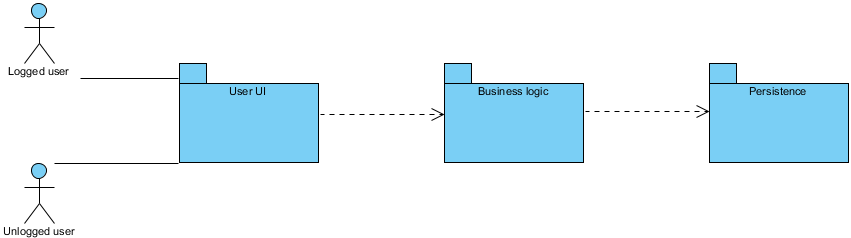
\includegraphics[width=\linewidth]{./images/basic-package}
\caption[Basic package]{Basic package diagram}
\label{fig:basic-package}
\end{figure}

QUESTO è VECCHIO
\part{Architecture description}
\section{JEE architecture overview}
Before focusing on our application's architecture we want to briefly explain the JEE architecture.

\begin{figure}[h]
\centering
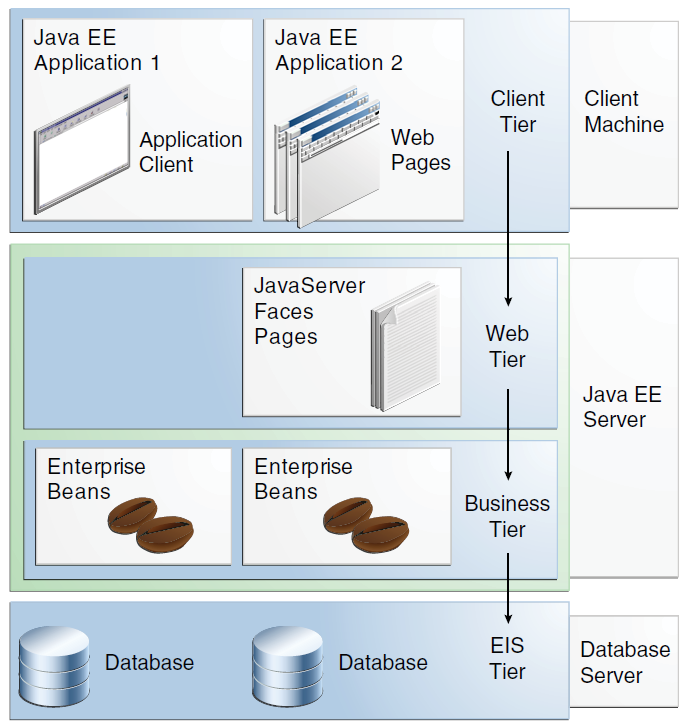
\includegraphics[width=\linewidth]{./images/JEE-arch}
\caption[JEE architecture]{JEE achitecture}
\label{fig:JEE-arch}
\end{figure}

As shown in figure \ref{fig:JEE-arch} JEE is divided in four tier:
\begin{itemize}
\item Client tier: containing Application Client and Web Pages it is the layer that directly interacts with the actors. As our project will be a web application the client will use a web browser to access pages.
\item Web tier: it contains the dynamic web pages that needs to be elaborated. This tier receives the requests from the client tier and forwards the pieces of data collected to the business tier waiting for processed data to be sent (eventually formatted) to the client tier.
\item Business tier: it contains the Java Beans, which are the elements that control the business logic of the application.
\item EIS tier: it contains the data source. In our case it is the database allowed to store all the relevant data and to retrieve them.
\end{itemize}

\section{Identifying sub-systems}
At this phase of the project we adopt a top-down approach to identify the main components of the system, once identified the sub-systems we will use a bottom-up approach to create more reusable components. We start by diving our system into smaller sub systems in order to better identify the various groups of functionalities and their interactions.

As depicted in figure \ref{fig:subsystems} the system is divided into three main packages, each with his own sub systems:
\begin{itemize}
\item User interface:
\begin{itemize}
\item Login page
\item Sign up page
\item Calendar page
\item Search page
\item Notification viewer
\end{itemize}

\item Business logic:
\begin{itemize}
\item Login manager
\item Sign up manager
\item Calendar manager
\item Search manager
\item Notification manager
\item Forecast manager
\end{itemize}

\item Persistence:
\begin{itemize}
\item Entity manager
\end{itemize}
\end{itemize}

\begin{figure}[h]
\centering
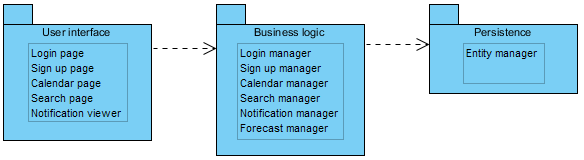
\includegraphics[width=\linewidth]{./images/sub-systems}
\caption[Subsystems]{System's packages and main components}
\label{fig:subsystems}
\end{figure}

\clearpage
\part{Persistent data management}
\section{Conceptual design}
\section{Logical design}
\subsection{ER restructuration}
RESTRUCTURATION IN INGLESE NON ESISTE
\subsection{Translation to logical model}

\clearpage
\part{User Experience}
\section{UX1}
\section{UX...n}

\clearpage
\part{BCE diagrams}
\section{Entity overview}
\section{BCE 1}
\section{BCE...n}
\section{User}
\subsection{BCE u1}
\subsection{BCE u...n}

\clearpage
\part{Sequence diagrams}
\section{SD1}
\section{SD..n}

\clearpage
\part{Final considerations}

\clearpage
\tableofcontents
\end{document}